\documentclass[a4paper,oneside,DIV=12,12pt]{scrartcl}

\usepackage{graphicx}

\usepackage{fontspec}
\setmainfont{PT Serif}
\setsansfont{PT Sans}
\setmonofont{PT Mono}

\usepackage{unicode-math}
\setmathfont{PT Serif}

\usepackage{microtype}

\usepackage{polyglossia}
\setmainlanguage{ukrainian}

% \usepackage{indentfirst}

% Table typesetting
\usepackage{booktabs}

\usepackage{array}
\newcolumntype{v}[1]{>{\raggedright\arraybackslash\hspace{0pt}}p{#1}}
\newcolumntype{n}[1]{>{\raggedleft\arraybackslash\hspace{0pt}}p{#1}}

\usepackage{multirow}
%

\usepackage{xcolor}

\usepackage{hyperref}
\hypersetup{
	colorlinks      = false,%
	linkbordercolor = blue,%
	pdfborderstyle  = {/S/U/W 1},%
}

\usepackage{enumitem}
\setlist[itemize]{label=—}

% Missing figure
\usepackage{todonotes}
%

\newcommand{\progname}{tinyplot}

\newcommand{\theprojcode}{PLOTSCRIPT}
\newcommand{\theprojrev}{00}
\newcommand{\thedoctype}{PRD}
\newcommand{\thedocnum}{000}
\newcommand{\thedocfullcode}{\theprojcode-\theprojrev-\thedoctype-\thedocnum}
\newcommand{\printdocfullcode}{\thedocfullcode}
\newcommand{\theversion}{2017-11-29-000}

\newcommand{\flagname}[1]{\texttt{#1}}
\newcommand{\cmdtoolname}[1]{\texttt{#1}}

\begin{document}
	\begin{titlepage}
	\begin{center}
		\vspace*{\fill}
			Технічне завдання\\
			на створення програмного продукту\\
			для побудови графіків
			
		\vspace*{\fill}
	\end{center}
	Кодова назва проекту: \theprojcode\\
	Код документу: \printdocfullcode\\
	Версія: \theversion\\
	\end{titlepage}
	
	\tableofcontents
	\newpage
	
	\section{Терміни та визначення}
		\subsection{Загальні терміни}
			Перелік загальних термінів, що використовуються у даному документі, їх скорочень та визначень, наведений у табл.~\ref{tab:general-definitions}.
			\begin{table}[!htbp]
			\centering
				\begin{tabular}{v{0.3\textwidth}lv{0.45\textwidth}}
					\toprule
						Термін                          & Скорочення & Значення\\
					\midrule
						Варіанти використання           & ВВ         & Див. посилання.\\
						Діаграма варіантів використання & ДВВ        & Див. посилання.\\
						Програмний продукт              & ПП         & Програма \progname, вимоги до~якої наведені у~даному документі.\\
						Технічне завдання               & ТЗ         & Документ, що описує вимоги до предмета розробки. Даний документ.\\
					\bottomrule
				\end{tabular}
			\caption{Перелік загальних термінів}
			\label{tab:general-definitions}
			\end{table}

		\subsection{Технічні терміни}
			Перелік технічних термінів, що використовуються у даному документі, їх скорочень та визначень, наведений у табл.~\ref{tab:tech-definitions}.
			\begin{table}[!htbp]
			\centering
				\begin{tabular}{v{0.3\textwidth}lv{0.45\textwidth}}
					\toprule
						Термін             & Скорочення & Значення\\
					\midrule
						Легенда            & —          & Розшифровка умовних позначень на~науковій графіці.\\
						Наукова графіка    & НГ         & Наочне зображення об'єктів наукових досліджень; графічна обробка результатів розрахунків.\\
						Операційна система & ОС         & \\
					\bottomrule
				\end{tabular}
			\caption{Перелік технічних термінів}
			\label{tab:tech-definitions}
			\end{table}

	\section{Загальні положення}
		\subsection{Призначення документу}
			
			Дане ТЗ призначене для використання у якості керівництва під час процесу розробки ПП. Задача ТЗ полягає в тому, щоб встановити чіткі вимоги до можливостей, які повинні бути надані розробленим продуктом, а також бути документальною базою для врегулювання можливих розбіжностей між Замовником і~Виконавцем.

			У даному документі представлений повний набір вимог до ПП, які необхідно реалізувати. При реалізації необхідно виконати роботи у повному об'ємі та~у~вказані терміни, які зазначенні в даному документі. Всі неточності, виявлені у~ТЗ після його утвердження, повинні бути узгоджені.

		\subsection{Цілі створення програмного продукту}

			З точки зору клієнтів створення ПП повинно досягти таких цілей:
			\begin{itemize}
				\item спростити побудову НГ на основі існуючих даних для клієнта;
				\item зменшити час на побудову НГ;
				\item отримати зображення НГ для подальшого використання.
			\end{itemize}

			Таким чином, при розробці ПП ставляться такі цілі:
			\begin{itemize}
				\item реалізація можливості побудови НГ на основі координатних точок;
				\item інтеграція можливості зчитування координатних точок з текстового файлу;
				\item реалізація можливості виведення результату у графічному файлі.
			\end{itemize}

		\subsection{Основні функціональні можливості програмного продукту}

			ПП повинен включати такі основні функціональні можливості:
			\begin{enumerate}
				\item Зчитування текстового файлу, який містить координатні точки.
				\item Побудова НГ на основі вхідних даних.
				\item Виведення побудованих НГ у вигляді графічного зображення.
				\item Попередній перегляд побудованої НГ.
				\item Побудова декількох графіків одночасно.
				\item Встановлення назв осей абсцис та ординат НГ.
				\item Встановлення ціни поділки НГ.
				\item Встановлення граничних значень на осях OX і~OY, у межах яких зображається НГ.
			\end{enumerate}
			
		\subsection{Прийом результату роботи}
			Для успішного прийому результатів роботи необхідно, щоб розробники ПП виконали усі основні функціональні вимоги, що вказані в~даному~ТЗ та дотримались термінів здачі готового продукту.
			
			У разі невідповідності будь-якої з вимог, умови подальшої співпраці узгоджуються сторонами у встановленому порядку згідно з умовами, поставленими у нормативних документах.

	\section{Функціональні вимоги}
		\subsection{Діаграми варіантів використання}
		На діаграмах представлені основні ВВ ПП, детальний опис яких можна знайти в п.~\ref{ssec:use-case-description}. На рис.~\ref{fig:client-use-case-diagram} зображена діаграма варіанту використання побудови графіка.
		
		\begin{figure}[!htbp]
		\centering
			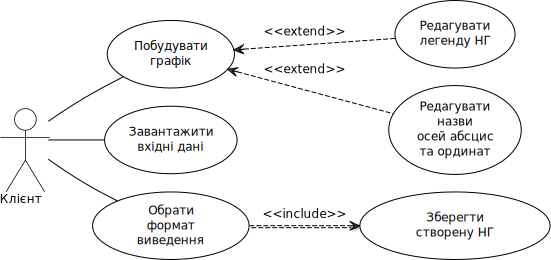
\includegraphics[width = \textwidth]{assets/use-case-diag-01.pdf}
		\caption{Діаграма варіантів використання}
		\label{fig:client-use-case-diagram}
		\end{figure}

		\subsection{Опис варіантів використання}
			\label{ssec:use-case-description}

		\subsubsection{Опис основних можливостей для клієнта}
		
			При використанні ПП клієнту повинні бути надані такі основні можливості:
			\begin{enumerate}
				\item Будувати двовимірний графік у прямокутній системі координат.
				\item Завантажувати вхідні дані зі спеціального файлу.
				\item Зберігати створену НГ.
				\item Редагувати назви осей абсцис та ординат.
				\item Редагувати ціну поділки.
				\item Обирати формат виведення готової НГ.
			\end{enumerate}

		\subsection{Додаткові функціональні вимоги}
			При використанні ПП клієнту можуть бути надані такі додаткові можливості:
			\begin{enumerate}
				\item Виведення інформації щодо використання команд при запуску з параметром \verb|--help|. 
				\item Вибір формату збереження готової НГ.
				\item Підтримка декількох текстових форматів (які обговорюються під час одного з етапів реалізації ПП та вибираються в залежності від можливостей розробників) для вводу даних.
				\item Редагування легенди НГ.
			\end{enumerate}

	\section{Нефункціональні вимоги}
		\subsection{Інтерфейс користувача}
			Даний ПП повинен мати інтерфейс командного рядка, що означає можливість запуску та налаштування ПП з командного рядка, що підтримується програмним продуктом. В свою чергу, це зумовлює такі уточнення:
			\begin{enumerate}
				\item Система націлена на роботу в командних рядках \cmdtoolname{cmd}, \cmdtoolname{bash}, \cmdtoolname{dash}, \cmdtoolname{csh}.
				\item Кодування тексту~— UTF-8 без BOM.
			\end{enumerate}

		\subsection{Підтримка операційних систем}

			ПП повинен коректно працювати в наступних операційних системах:
			\begin{enumerate}
				\item Windows 7 та вище.
				\item Ubuntu 14.04~LTS, 16.04~LTS, 17.04 та вище.
				\item Debian 9 та вище.
				\item Fedora 26 та вище.
			\end{enumerate}
			
		\subsection{Установка}
			Якщо для коректної роботи ПП існує потреба встановлення додаткових програм, файлів, бібліотек тощо, користувач повинен бути про це попереджений за допомогою керівництва користувача або відповідного повідомлення під час роботи. Рекомендується автоматичне встановлення необхідних утиліт для коректної роботи програми.

		\subsection{Вимоги до продуктивності}
			До продуктивності ПП встановлюються такі вимоги:
			\begin{enumerate}
				\item ПП повинен стабільно працювати з великою кількістю координатних точок (більше 40).
				\item ПП повинен створювати вихідну НГ не довше 30~секунд.
				\item Час створення декількох НГ повинен бути обмежений лінійно, тобто для створення двох НГ не повинно займати не більше ніж $2 \times 30 = 60$~секунд.
			\end{enumerate}

	\section{Вимоги до прийому та здачі проекту}

		Розробник повинен надати такий комплект документів під час здачі проекту:
		\begin{enumerate}
			\item Початковий код ПП.
			\item Виконавчі файли.
			\item Тест-план.
			\item Тестові сценарії.
			\item Баг-репорти.
			\item Керівництво користувача.
		\end{enumerate}

% [1]: https://ru.wikipedia.org/wiki/Use_case "Сценарий использования"
% [2]: https://ru.wikipedia.org/wiki/UML "UML"


\end{document}